%% LyX 2.3.6.1 created this file.  For more info, see http://www.lyx.org/.
%% Do not edit unless you really know what you are doing.
\documentclass[english]{article}
\usepackage[T1]{fontenc}
\usepackage[latin9]{inputenc}
\usepackage{geometry}
\geometry{verbose,tmargin=2.5cm,bmargin=2.5cm,lmargin=2.5cm,rmargin=2.5cm}
\usepackage{graphicx}

\makeatletter

%%%%%%%%%%%%%%%%%%%%%%%%%%%%%% LyX specific LaTeX commands.
%% Because html converters don't know tabularnewline
\providecommand{\tabularnewline}{\\}

\makeatother

\usepackage{babel}
\begin{document}
{[}SPLIT\_HERE{]}
\begin{enumerate}
\item \textbf{{[}DHS/PRELIM/9597/2019/P1/Q1{]} }

The file \texttt{IOI19.TXT} stores the scoreboard of the 31st International
Olympiad in Informatics (IOI) held in Baku, Azerbaijan from 4 to 11
August 2019. The first line contains the header with contestant's
rank, name, team (country), and overall score. The remaining lines
contain the corresponding data. IOI 2019 eventually awarded 28 Gold,
54 Silver and 81 Bronze medals. A country typically sends up to 4
contestants to participate in IOI. 

\subsection*{Task 1.1 }

Determine the top 3 teams in the competition and display their country
names as well as the number of Gold, Silver and Bronze medals attained.
Teams which are tied will be ordered by their country names in alphabetical
order and will share the same rank. 

Sample output: 

\texttt{Top 3 teams: }

\texttt{1 ABC 4G }

\texttt{2 DEF 3G1S }

\texttt{2 GHI 3G1S }

\texttt{4 JKL 2G1S1B }

\texttt{4 MNO 2G1S1B }

\subsection*{Evidence 1 }

Program code. \hfill{}{[}9{]}

\subsection*{Evidence 2 }

Screenshot. \hfill{} {[}1{]}

\subsection*{Task 1.2 }

Write program code to prompt a user to enter a team name and display
the results of its participants. Participants who did not receive
a medal will be denoted with \texttt{P}. The program will terminate
when a user enters the text string \texttt{'ZZZ'} (without the quotes). 

Sample interaction: 

\texttt{Enter team: SGP }

\texttt{Eu-Shaun Leong G }

\texttt{Lee Jeffrey Chun Hean S }

\texttt{Benson Zhan Li Lin B }

\texttt{Daniel Zhenghao Choo P }

\texttt{Enter team: ZZZ }

\texttt{Bye }

\subsection*{Evidence 3}

Program code. \hfill{} {[}4{]}

\subsection*{Evidence 4 }

Screenshot. \hfill{}{[}1{]}

{[}SPLIT\_HERE{]}
\item \textbf{{[}DHS/PRELIM/9597/2019/P1/Q2{]} }

Dubbed first of its kind globally, the Singapore Quick Response Code
(SGQR) is an infrastructure-light technology that will help to simplify
QR e-payments in Singapore for both consumers and merchants. 

The SGQR is based on the QR Code Specification for Payment System
- Merchant-Presented Mode standard issued by EMVCo, which has the
benefits of international interoperability, multi-tenancy of QR schemes
and non-sensitive data presented for payments. 

According to the specification, the parsed SGQR text string contains
data items, with each data item adhering to the following structure:
id, length, value. Two such data items are highlighted in bold in
the following diagram: 
\begin{center}
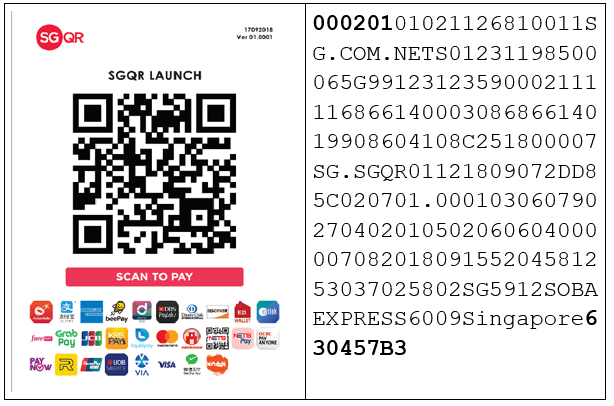
\includegraphics[width=0.5\paperwidth]{C:/Users/Admin/Desktop/Github/question_bank/LyX/static/img/9597-DHS-2019-P1-Q2}
\par\end{center}

Thus for the first data item \texttt{\textbf{000201}}, \texttt{00}
is the id, \texttt{02} is the length, and \texttt{01} is the value. 

And for the last data item \texttt{\textbf{630457B3}}, \texttt{63}
is the id, \texttt{04} is the length, and \texttt{57B3} is the value. 

The value \texttt{57B3} is also a hexdecimal number to verify the
integrity of the SGQR data. 

\subsection*{Task 2.1 }

Write program code to extract the last data item of the SGQR stored
in \texttt{SGQR.TXT}. For the example above, it will be the data item
with id 63 and length 4 i.e. 630457B3. 

\subsection*{Evidence 5 }

Program code. \hfill{} {[}3{]}

\subsection*{Evidence 6 }

Screenshot. \hfill{} {[}1{]}

\subsection*{Task 2.2 }

Write a \texttt{hex2oct} function which takes in a hexadecimal number
string and returns its equivalent octal number string. For example
\texttt{hex2oct('A')} returns \texttt{'12'}. You may not use Python's
built in \texttt{int(num, 8)}, \texttt{int(num, 16)}, \texttt{bin()},
\texttt{oct()} or \texttt{hex()} functions. Use the hexadecimal number
string \texttt{'4F63A'} to to test your program code. 

Hint: One hexadecimal digit can be expressed as four binary digits
and one octal digit can be expressed as three binary digits. 

\subsection*{Evidence 7 }

Program code. \hfill{}{[}5{]}

\subsection*{Evidence 8 }

Screenshot. \hfill{}{[}1{]}

\subsection*{Task 2.3 }

Write program code to perform input validation for a hexadecimal number
string. Test your program with suitable test data. 

\subsection*{Evidence 9 }

Program code. \hfill{}{[}3{]}

\subsection*{Evidence 10 }

Screenshots. \hfill{}{[}2{]}

{[}SPLIT\_HERE{]}
\item \textbf{{[}DHS/PRELIM/9597/2019/P1/Q3{]} }

From 2021 onwards, the Primary School Leaving Exam (PSLE) will be
scored with wider bands, replacing the current T-scores. 

Each subject will be scored using 8 bands known as Achievement Levels
(AL), with AL 1 being the best score and AL 8 being the lowest score.
The student\textquoteright s PSLE Score will be the sum of the four
subject scores. The PSLE Score will range from 4 (best) to 32. 
\begin{center}
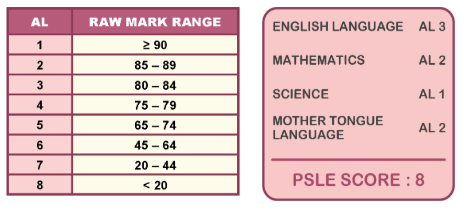
\includegraphics[width=0.5\paperwidth]{C:/Users/Admin/Desktop/Github/question_bank/LyX/static/img/9597-DHS-2019-P1-Q3}
\par\end{center}

Secondary 1 posting will continue to be based on academic merit, using
the PSLE Score. 

Each student will submit a list of 6 schools in order of preference.
If two students with the same score are being considered for the last
place in a school, the following tie-breakers will be used: 
\begin{itemize}
\item Citizenship - priority given to Singapore Citizens (SC), then Singapore
Permanent Residents (PR), then International Students (IS) 
\item Choice order of schools - priority given to the student who indicates
a certain school as a higher choice 
\item Computerised balloting 
\end{itemize}
The file \texttt{PSLE21.txt} contains the application information
of 400 Primary 6 students of a primary school with the following structure:

\texttt{<StudentID>,<EnglishLanguageMark>,<MathematicsMark>,<ScienceMark>,<MotherTongueLangueMark>,<Citizenship>,<SchoolChoice1>,<SchoolChoice2>
,<SchoolChoice3> }

You may assume that in this school all students study subjects at
the standard level. Also, all of them have made up their mind to only
apply to 3 schools of their choice. If a student is unable to get
admission to a school of their choice, they will be posted to SchoolD.

It is decided to process and store the following application information
about the student in 4 linked lists. Each linked list pertain to the
vacancy positions of the 4 schools. Schools A, B and C have 120, 150
and 80 available places. The data to be stored in each linked list
node include: PSLE score, student ID, citizenship and the 3 school
choices. 

\subsection*{Task 3.1 }

Write program code to read in and store the contents of the file \texttt{PSLE21.txt}
in a dictionary \texttt{students} with key \texttt{StudentID} and
value the computed PSLE score, citizenship and three school choices.
Display the first 10 dictionary entries in \texttt{students}. 

\subsection*{Evidence 11}

Program code. \hfill{}{[}6{]}

\subsection*{Evidence 12 }

Screenshot for first 10 dictionary entries in \texttt{students}.\hfill{}
{[}1{]}

\subsection*{Task 3.2 }

Using OOP where appropriate, write program code to declare and initialise
the necessary classes. Insert the 400 students from the \texttt{students}
dictionary in Task 3.1 to the appropriate linked lists in your main
program driver code. 

\subsection*{Evidence 13 }

Program code. \hfill{}{[}16{]}

\subsection*{Evidence 14 }

Screenshots for the first 5 entries in each linked list. \hfill{}{[}4{]}

\subsection*{Task 3.3 }

Students \texttt{P351} and \texttt{P365} who were previously Singapore
Permanent Residents (PR) have successfully become Singapore Citizens
(SC). Write the necessary program code to update their citizenship
status and new secondary 1 posting order. 

\subsection*{Evidence 15}

Program code. \hfill{}{[}5{]}

\subsection*{Evidence 16 }

Screenshots. \hfill{}{[}2{]}

\subsection*{Task 3.4}

Student \texttt{P286} has decided to emigrate to another country with
his/her parents. Write the necessary program code to remove him/her
from his/her existing allocation and perform the necessary adjustments
to fill up the vacancy. 

\subsection*{Evidence 17}

Program code. \hfill{}{[}5{]}

\subsection*{Evidence 18 }

Screenshot.\hfill{} {[}1{]}

{[}SPLIT\_HERE{]}
\item \textbf{{[}DHS/PRELIM/9597/2019/P1/Q4{]} }

The Viola-Jones object detection algorithm, named after two computer
vision researchers Paul Viola and Michael Jones, uses integral images
to detect the presence of facial features in an image efficiently. 

An integral image (also known as a summed-area table) is the name
of both a data structure and an algorithm used to obtain this data
structure. It uses a quick and efficient way to calculate the sum
of pixel values in a rectangular part of an image. 

In an integral image, the value of each point is the sum of all pixels
above and to the left, including the target pixel: 
\begin{center}
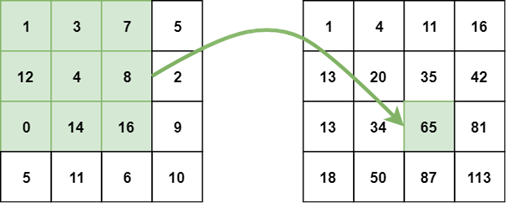
\includegraphics[width=0.5\paperwidth]{C:/Users/Admin/Desktop/Github/question_bank/LyX/static/img/9597-DHS-2019-P1-Q4-1}
\par\end{center}

The integral image can be calculated in a single pass over the original
image. This reduces summing the pixel intensities within a rectangle
into only three operations with four numbers, regardless of rectangle
size: 
\begin{center}
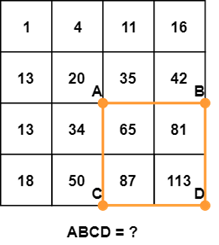
\includegraphics[width=0.25\paperwidth]{C:/Users/Admin/Desktop/Github/question_bank/LyX/static/img/9597-DHS-2019-P1-Q4-2}
\par\end{center}

The sum of pixels in the rectangle ABCD can be derived from the values
of points A, B, C, and D, using the formula $D-B-C+A$. It is easier
to understand this formula visually:

Note that subtracting both B and C means that the area defined with
A has been subtracted twice, so we need to add it back again. 

Thus $D-B-C+A=113-50-42+20=41$. 
\begin{center}
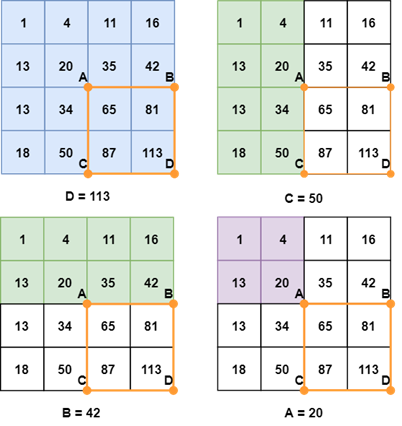
\includegraphics[width=0.5\paperwidth]{C:/Users/Admin/Desktop/Github/question_bank/LyX/static/img/9597-DHS-2019-P1-Q4-3}
\par\end{center}

\subsection*{Task 4.1 }

Write an \texttt{integral\_image()} function which reads in the data
from the file \texttt{IMAGE1.IN} into a 2D array and computes and
outputs the integral image to a file \texttt{IMAGE1.OUT} using the
algorithm described above, and also displays the result of $D-B-C+A$
to the screen. 

\subsection*{Evidence 19}

Program code. \hfill{} {[}13{]}

\subsection*{Evidence 20}

Screenshots of \texttt{IMAGE1.OUT} and output of $D-B-C+A$. \hfill{}{[}2{]}

\subsection*{Task 4.2}

Write a \texttt{magic()} function which is a generalisation of your
\texttt{integral\_image()} function which will work for any $m\times n$
rectangular 2D array and any rectangle ABCD.

Programmatically randomise your image with suitable values ($m,n\geq8$)
in \texttt{IMAGE2.IN} and work your magic on this pseudo-randomly
generated file to produce \texttt{IMAGE2.OUT} and the updated computed
value of $D-B-C+A$. 

\subsection*{Evidence 21}

Program code. \hfill{}{[}13{]}

\subsection*{Evidence 22 }

Screenshots of \texttt{IMAGE2.OUT} and output of $D-B-C+A$. \hfill{}{[}2{]}

{[}SPLIT\_HERE{]}
\item \textbf{{[}DHS/PRELIM/9597/2019/P2/Q1{]} }

The following Gantt chart shows the key tasks involved in a data science
project for a product recommendation engine based on customers' past
purchase patterns.
\noindent \begin{center}
\begin{tabular}{|c|l|c|c|c|c|c|c|c|c|c|c|c|c|c|c|c|c|c|c|c|c|c|}
\hline 
AID & Activity & \multicolumn{21}{c|}{Week}\tabularnewline
\hline 
A & Understand the problem & X & X &  &  &  &  &  &  &  &  &  &  &  &  &  &  &  &  &  &  & \tabularnewline
\hline 
B & Review with team &  &  & X &  &  &  &  &  &  &  &  &  &  &  &  &  &  &  &  &  & \tabularnewline
\hline 
C & Make problem statement &  &  & X &  &  &  &  &  &  &  &  &  &  &  &  &  &  &  &  &  & \tabularnewline
\hline 
D & Define scope of work &  &  & X &  &  &  &  &  &  &  &  &  &  &  &  &  &  &  &  &  & \tabularnewline
\hline 
E & Identify suitable algorithms &  &  &  & X &  &  &  &  &  &  &  &  &  &  &  &  &  &  &  &  & \tabularnewline
\hline 
F & Collect data &  &  & X & X & X & X & X & X &  &  &  &  &  &  &  &  &  &  &  &  & \tabularnewline
\hline 
G & Clean data &  &  & X & X & X & X & X & X &  &  &  &  &  &  &  &  &  &  &  &  & \tabularnewline
\hline 
H & Exploratory data analysis &  &  &  &  & X & X &  &  &  &  &  &  &  &  &  &  &  &  &  &  & \tabularnewline
\hline 
I & Develop use cases &  &  &  &  &  & X & X &  &  &  &  &  &  &  &  &  &  &  &  &  & \tabularnewline
\hline 
J & Present use cases &  &  &  &  &  &  &  & X &  &  &  &  &  &  &  &  &  &  &  &  & \tabularnewline
\hline 
K & Analyse full data &  &  &  &  &  &  &  &  & X & X & X &  &  &  &  &  &  &  &  &  & \tabularnewline
\hline 
L & Develop proof of concept &  &  &  &  &  &  &  &  &  &  &  & X & X & X &  &  &  &  &  &  & \tabularnewline
\hline 
M & Get customer approval &  &  &  &  &  &  &  &  &  &  &  &  &  &  & X &  &  &  &  &  & \tabularnewline
\hline 
N & Build final models &  &  &  &  &  &  &  &  &  &  &  &  &  &  &  & X & X & X &  &  & \tabularnewline
\hline 
O & Deploy models &  &  &  &  &  &  &  &  &  &  &  &  &  &  &  &  &  &  & X & X & \tabularnewline
\hline 
P & Sign off &  &  &  &  &  &  &  &  &  &  &  &  &  &  &  &  &  &  &  &  & X\tabularnewline
\hline 
\end{tabular}
\par\end{center}

A project manager often uses both PERT chart and Gantt chart to illustrate
and manage a project workflow. 
\begin{enumerate}
\item Give one benefit and one limitation of using a Gantt chart to depict
a project workflow?\hfill{} {[}2{]}
\item {}
\begin{enumerate}
\item Construct a PERT chart to depict the project work flow.\hfill{} {[}4{]}
\item State the critical path and the minimum project completion time. \hfill{}{[}2{]}
\item Explain and give an example of a dependent activity.\hfill{} {[}2{]}
\item Explain and give an example of a concurrent activity. \hfill{}{[}2{]}
\item Indicate in your PERT chart and justify a suitable dummy activity.
\hfill{}{[}2{]}
\item Give an example to show your understanding of float or slack time.\hfill{}
{[}2{]}
\end{enumerate}
\item The project manager needs to include a documentation activity and
a cybersecurity activity to the project. Justify the significance
of these activities and show how these can be included in your PERT
chart. Explain any implications to the critical path and projection
completion time. \hfill{}{[}5{]}
\item The project team would inadvertently have access to some restricted
customer purchase information. Give two ethical considerations related
to the privacy of data and suggest possible mitigation measures.\hfill{}
{[}4{]}
\end{enumerate}
The following shows sample interaction snippets of an interactive
exploratory data analysis session. 
\begin{center}
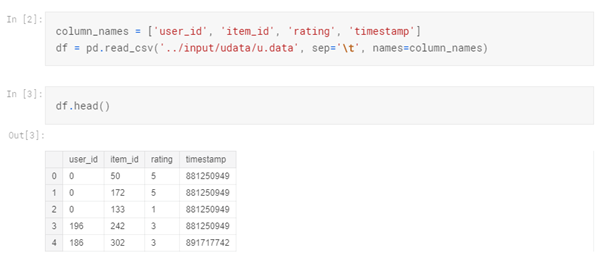
\includegraphics[width=0.65\paperwidth]{C:/Users/Admin/Desktop/Github/question_bank/LyX/static/img/9597-DHS-2019-P2-Q1-1}
\par\end{center}

\begin{center}
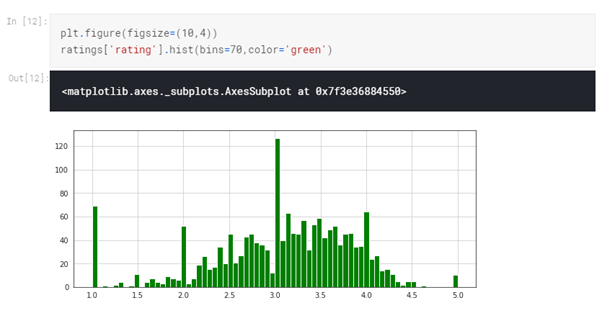
\includegraphics[width=0.65\paperwidth]{C:/Users/Admin/Desktop/Github/question_bank/LyX/static/img/9597-DHS-2019-P2-Q1-2}
\par\end{center}
\begin{enumerate}
\item[(e)]  {}
\begin{enumerate}
\item State the interface used and justify why this is the most appropriate
form of user interaction. \hfill{}{[}3{]}
\item The data analysis team is deciding on whether to perform the analysis
online in a cloud infrastructure or to process all data on a local
computer. What are two factors to consider in arriving at this decision?
\hfill{}{[}2{]}
\item Evaluate the pros and cons of each approach and make a recommendation
with reason(s) to the project team. \hfill{}{[}5{]}
\end{enumerate}
\item[(f)]  Given the relationship: bit rate = baud rate {*} voltage (\# bits
per signal)
\begin{enumerate}
\item Explain the difference between baud rate and bit rate. \hfill{}{[}2{]}
\item The following voltage levels expressed in volts are chosen to encode
bits:

-6.0, -4.5, -3.0, -1.5, +1.5, +3.0, +4.5, +6.0

How many bits represent these voltages?\hfill{} {[}1{]}
\item For the above voltages, write down one possible set of corresponding
bit patterns.\hfill{} {[}1{]}
\item If the baud rate of the line is 900 baud what is the bit rate for
the voltage levels?\hfill{} {[}1{]}
\end{enumerate}
{[}SPLIT\_HERE{]}
\end{enumerate}
\item \textbf{{[}DHS/PRELIM/9597/2019/P2/Q2{]} }
\begin{enumerate}
\item Given an array of integers, devise an algorithm for a function \texttt{FindLargest}
that arranges them in order to return the largest possible integer.
For example, given {[}10, 7, 76, 415{]}, your algorithm should return
77641510.\hfill{} {[}5{]}
\item Given an array of integers, devise an algorithm for a function \texttt{MultiplyNotMe}
that returns a new array such that each element at index i of the
new array is the product of all the numbers in the original array
except the one at i. For example, given {[}1, 2, 3, 4, 5{]}, your
algorithm should return {[}120, 60, 40, 30, 23{]}.\hfill{} {[}5{]}
\end{enumerate}
{[}SPLIT\_HERE{]}
\item \textbf{{[}DHS/PRELIM/9597/2019/P2/Q3{]} }
\begin{enumerate}
\item Given a binary search tree of positive integers, devise an algorithm
\texttt{FindFloorCeiling} to find the floor and ceiling of a given
positive integer k. The floor Is the highest element in the tree less
than or equal to an integer, while the ceiling is the lowest element
in the tree greater than or equal to an integer. If either value does
not exist, return -1. \hfill{}{[}5{]}
\item Given a sorted array, devise an algorithm \texttt{MakeBalancedBST}
to convert it into a height-balanced binary search tree. \hfill{}{[}5{]}
\end{enumerate}
{[}SPLIT\_HERE{]}
\item \textbf{{[}DHS/PRELIM/9597/2019/P2/Q4{]} }

Blackjack is a two-player card game whose rules are as follows:
\begin{itemize}
\item The player and then the dealer are each given two cards. 
\item The player can then \textquotedbl hit\textquotedbl , or ask for
arbitrarily many additional cards, so long as their total does not
exceed 21. 
\item The dealer must then hit if their total is 16 or lower, otherwise
pass. 
\item Finally, the two compare totals, and the one with the greatest sum
not exceeding 21 is the winner.
\end{itemize}
For this problem, cards values are counted as follows: each card between
2 and 10 counts as their face value, face cards count as 10, and aces
count as 1. 
\begin{enumerate}
\item Express the above blackjack game flow using a program flowchart. \hfill{}{[}4{]}
\item Given perfect knowledge of the sequence of cards in the deck, devise
an efficient algorithm that maximises the player's score (i.e. wins
minus losses). \hfill{} {[}8{]}
\item Evaluate the efficiency of your algorithm for part (b). \hfill{}{[}3{]}
\end{enumerate}
{[}SPLIT\_HERE{]}
\item \textbf{{[}DHS/PRELIM/9597/2019/P2/Q5{]} }

A role playing game (RPG) uses object-oriented programming (OOP) to
store its game characters' data. A character, either a hero or a monster,
has a name, health, magic points and inventory. Each character also
has a \texttt{take\_damage()} and a \texttt{display()} method. 

The game also has a special type of character, a dragon, which also
has additional data \texttt{airSpeed} and \texttt{breathType}.
\begin{enumerate}
\item Draw a class diagram showing the relationship between the different
game characters. \hfill{}{[}4{]}
\item Using appropriate examples, explain the following terms:
\begin{enumerate}
\item encapsulation
\item inheritance
\item polymorphism \hfill{}{[}6{]}
\end{enumerate}
\item Using suitable examples, explain why OOP is a preferred programming
paradigm in game development than a(n) imperative/procedural one.
\hfill{} {[}2{]}
\end{enumerate}
{[}SPLIT\_HERE{]}
\item \textbf{{[}DHS/PRELIM/9597/2019/P2/Q6{]} }

BuildingBloCS is Singapore's first/only/largest by Computing students
for Computing students and beyond national Computing education outreach
programme. In 2019, it comprises a series of workshops, talks, games,
projects showcase, programming quizzes, lucky draws and more (media
and entertainment very important). 

The organisers would like to apply what they learned in Computing
to manage workshop information using a relational database. 
\begin{itemize}
\item Each participant can register for one or more workshops 
\item Each workshop is conducted by one or more instructors 
\item Each workshop is also facilitated by one or more facilitators 
\end{itemize}
Due to Personal Data Protection Act (PDPA), it is decided to use an
alternative unique identifier as the primary key instead of collecting
participants' NRICs/FINs.

The normalised design requires a number of tables.
\begin{enumerate}
\item Draw an Entitiy-Relationship (E-R) diagram that shows these tables
and the relationships between them. \hfill{} {[}4{]}
\item Suggest and justify a suitable primary key candidate other than NRIC/FIN.
\hfill{} {[}2{]}
\item A table description can be expressed as:

\texttt{TableName(Attribute1, Attribute2, Attribute3, \dots )}

The primary key is indicated by underlining one or more attributes.

Derive the table descriptions for the tables. \hfill{}{[}6{]}
\item There are some fields with missing or null values. Explain how these
arise and how a Database Management System (DBMS) may provide facilities
to ensure the information is appropriately managed. \hfill{}{[}3{]}
\end{enumerate}
{[}SPLIT\_HERE{]}
\end{enumerate}

\end{document}
